%\documentclass[t]{beamer}  % [t], [c], или [b] --- вертикальное выравнивание на слайдах (верх, центр, низ)
\documentclass{article} % Соотношение сторон

%графики
\usepackage{pgfplots}
\pgfplotsset{compat=1.9}


\usepackage{multicol}
\usepackage{mathrsfs}
\usepackage{booktabs}


%%% Работа с русским языком
\usepackage[T2A]{fontenc}			% кодировка
\usepackage[utf8]{inputenc}			% кодировка исходного текста
\usepackage[english,russian]{babel}	% локализация и переносы

%%% Дополнительная работа с математикой
\usepackage{amsmath,amsfonts,amssymb,amsthm,mathtools} % AMS
\usepackage{bm}

%%% Работа с картинками
\usepackage{graphicx}  % Для вставки рисунков
\setlength\fboxsep{3pt} % Отступ рамки \fbox{} от рисунка
\setlength\fboxrule{1pt} % Толщина линий рамки \fbox{}

\usepackage{braket} %Бракеты
\usepackage[version=4]{mhchem} 
\title{Лабораторная работа 3.3.5  \\
"Эффект Холла в металлах"}

\begin{document}

\maketitle
\subsection*{Цель:}
Измерение подвижности и концентрации носителей заряда в металлах
\subsection*{Оборудование:}
Электромагнит с источником питания, источник постоянного тока, микровольтметр,
амперметры, магнитометр, образцы из серебра и цинка.

\subsection*{Теоретические сведения}

Формула проводимости
\begin{equation}
\sigma = e n b
\end{equation}
$b$ -- подвижность, $n$ --
концентрация, $e$ -- элементарный заряд,
показывает что исследование электрической
проводимости проводников позволяет
определить произведение $nb$. Как мы
увидим ниже, исследование эффекта Холла
позволяет находить плотность носителей
$n$, после чего можно найти и их
подвижность $b$. Таким образом,
одновременное исследование электрической
проводимости и эффекта Холла позволяет
экспериментально находить важнейшие
параметры, определяющие состояние
электронов в металлах и полупроводниках.
Эффект Холла позволяет также определить
преобладающий тип проводимости —
электронный или дырочный.

Суть эффекта Холла состоит в следующем.
Пусть через однородную пластину металла
вдоль оси $x$ течёт ток $I$ (рис. 1).

Если эту пластину поместить в магнитное
поле, направленное по оси у, то между
гранями А и Б появляется разность
потенциалов. В самом деле, на электрон,
движущийся со скоростью $\langle
\vec \upsilon \rangle $ в
электромагнитном поле, действует сила
Лоренца:
\begin{equation}
    \vec F_\text{л} = -e\vec E - e
    \langle \vec \upsilon \rangle \times
    \vec B
\end{equation}
где $e$ — абсолютная величина
заряда электрона, $E$ — напряжённость
электрического поля, $B$ — индукция
магнитного поля. В нашем случае сила,
обусловленная вторым слагаемым,
направлена вдоль оси $z$:
\[
    F_B = e|\,\langle \upsilon_x
    \rangle\, |
    B
\]
Здесь $|\,\langle \upsilon_x \rangle\, |$ — абсолютная величина
дрейфовой скорости электронов вдоль оси
$x$, возникающая под действием внешнего
электрического поля.


Под действием этой силы электроны
отклоняются к грани Б, заряжая её
отрицательно (для простоты рассматриваем
только один тип носителей). На грани А
накапливаются нескомпенсированные
положительные заряды. Это приводит к
возникновению электрического поля $E_z$,
направленного от А к Б, которое
действует на электроны с силой $F_E =
eE_z$,
направленной против силы $F_B$. В
установившемся режиме сила $F_E$ 
уравновешивает силу $F_B$, И накопление
электрических зарядов на боковых гранях
пластины прекращается. Из условия
равновесия $F_B = F_E$ найдём
\begin{equation}
    E_z = |\, \langle \upsilon_x \rangle
    \, | B
\end{equation}
Поле $E_z$ даёт вклад в общее поле $E$, в
котором движутся электроны. С полем $E_z$ 
связана разность потенциалов
$U_{\text{АБ}}$ между
гранями А и Б:
\begin{equation}
    U_{\text{АБ}} = -E_z l = -
    |\,\langle \upsilon_x \rangle \, | B
    l
\end{equation}
В этом и состоит эффект Холла. Второе
слагаемое в силе Лоренца (2), с
которым связан эффект, часто называют
<<холловским>>.

Замечая, что сила тока
\begin{equation}
    I = ne| \, \langle \upsilon_x
    \rangle \, | l\cdot a,
\end{equation}
и объединяя (3) и (5), найдем ЭДС
Холла:
\begin{equation}
    \mathscr{E}_x = U_\text{АБ} = -
    \frac{IB}{nea} = -R_x \cdot
    \frac{IB}{a}
\end{equation}

Константа $R_x$ называется постоянной
Холла. Как видно из (6):
\[
R_x = \frac{1}{ne}
\]

\subsection*{Экспериментальная установка:}
Электрическая схема установки для
измерения ЭДС Холла представлена на рис.1.
\begin{figure}
    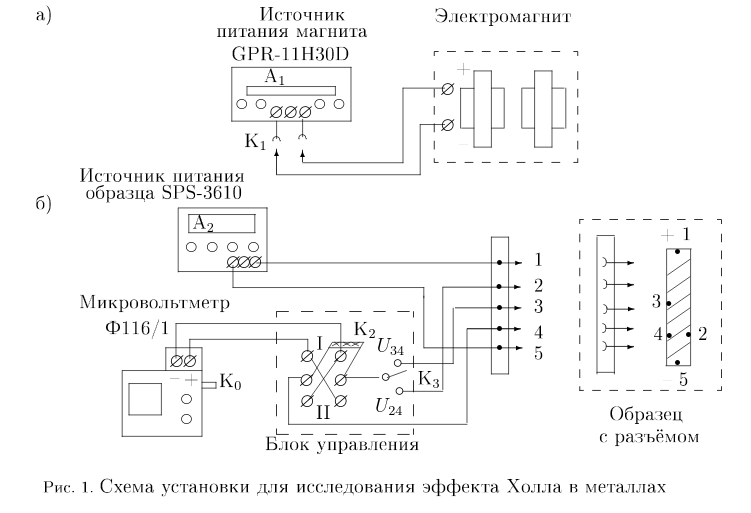
\includegraphics[width=0.725\linewidth]{Scheme.png} 
\end{figure}
В зазоре электромагнита (рис. 2а)
создаётся постоянное магнитное поле,
величину которого можно менять с помощью
источника питания электромагнита. Разъём
$\text{К}_1$ позволяет менять направление тока в
обмотках электромагнита. Ток питания
электромагнита измеряется амперметром
$\text{А}_1$. Градуировка магнита
проводится с помощью милливеберметра.

Металлические образцы в форме тонких
пластинок, смонтированные в специальных
держателях, подключаются к блоку питания
через разъём (рис. 2б). Ток через
образец регулируется реостатом $R_2$ и
измеряется амперметром $\text{А}_2$.

Для измерений ЭДС Холла используется
микровольтметр Ф116/1, в котором высокая
чувствительность по напряжению
сочетается с малой величиной тока,
потребляемого измерительной схемой:
минимальный предел измерения напряжения
составляет 1,5 мкВ, а потребляемый ток —
всего $10^{-8}$ А.

В образце с током, помещённом в зазор
электромагнита, между контактами 2 и 4
возникает холловская разность
потенциалов, которая измеряется с
помощью микровольтметра, если
переключатель $\text{К}_3$ подключён к точке 2
образца. При подключении $\text{К}_3$ к точке 3
микровольтметр измеряет омическое
падение напряжения $U_{34}$, вызванное
основным током через образец. При
нейтральном положении ключа входная цепь
микровольтметра разомкнута.

Ключ $\text{К}_2$ позволяет менять
полярность напряжения, поступающего на
вход микровольтметра.

Иногда контакты 2 и 4 вследствие
неточности подпайки не лежат на одной
эквипотенциали, и тогда напряжение между
ними связано не только с эффектом Холла,
но и с омическим падением напряжения,
вызванным протеканием основного тока
через образец. Измеряемая разность
потенциалов при одном направлении
магнитного поля равна сумме ЭДС Холла и
омического падения напряжения, а при
другом — их разности. В этом случае ЭДС
Холла $\mathscr{E}_x$ может быть определена как
половина алгебраической разности
показаний вольтметра, полученных для
двух противоположных направлений
магнитного поля в зазоре.

Можно исключить влияние омического
падения напряжения иначе, если при
каждом токе через образец измерять
напряжение $U_0$ между точками 2 и 4 в
отсутствие магнитного поля. При
фиксированном токе через образец это
дополнительное к ЭДС Холла напряжение
остаётся неизменным. От него следует (с
учётом знака) отсчитывать величину ЭДС
Холла:
\begin{equation}
    \mathscr{E}_x = U_{24} \pm U_0
\end{equation}
При таком способе измерения нет
необходимости проводить повторные
измерения с противоположным направлением
магнитного поля.

По знаку $\mathscr{E}_x$ можно определить характер
проводимости — электронный или дырочный.
Для этого необходимо знать направление
тока в образце и направление магнитного
поля.

Измерив ток $I$ в образце и напряжение
$U_{34}$ 
между контактами 3 и 4 в отсутствие
магнитного поля, можно, зная параметры
образца, рассчитать проводимость
материала образца по очевидной формуле:
\begin{equation}
    \sigma = \frac{I L_{34}}{U_{34} a
    l},
\end{equation}
где $L_{34}$ -- расстояние между
контактами 3 и 4, $a$ -- толщина
образца, $l$ -- его ширина.

\subsection*{Результаты измерений и обработка результатов}
\begin{center}
данные для калибровочной кривой электромагнита\\
\begin{tabular}{|l|l|}
B,mT  & Im,A   \\ \hline
123.3 & 0.1   \\\hline
356   & 0.29  \\\hline
597   & 0.49   \\\hline
705   & 0.6    \\\hline
976   & 0.9   \\\hline
1068  & 1.1   \\\hline
1107  & 1.2  \\\hline
\end{tabular}
\end{center}
Построим график зависимости $B(I_m)$ для того, чтобы в дальнейшем по нему считать B\\
\begin{figure}
    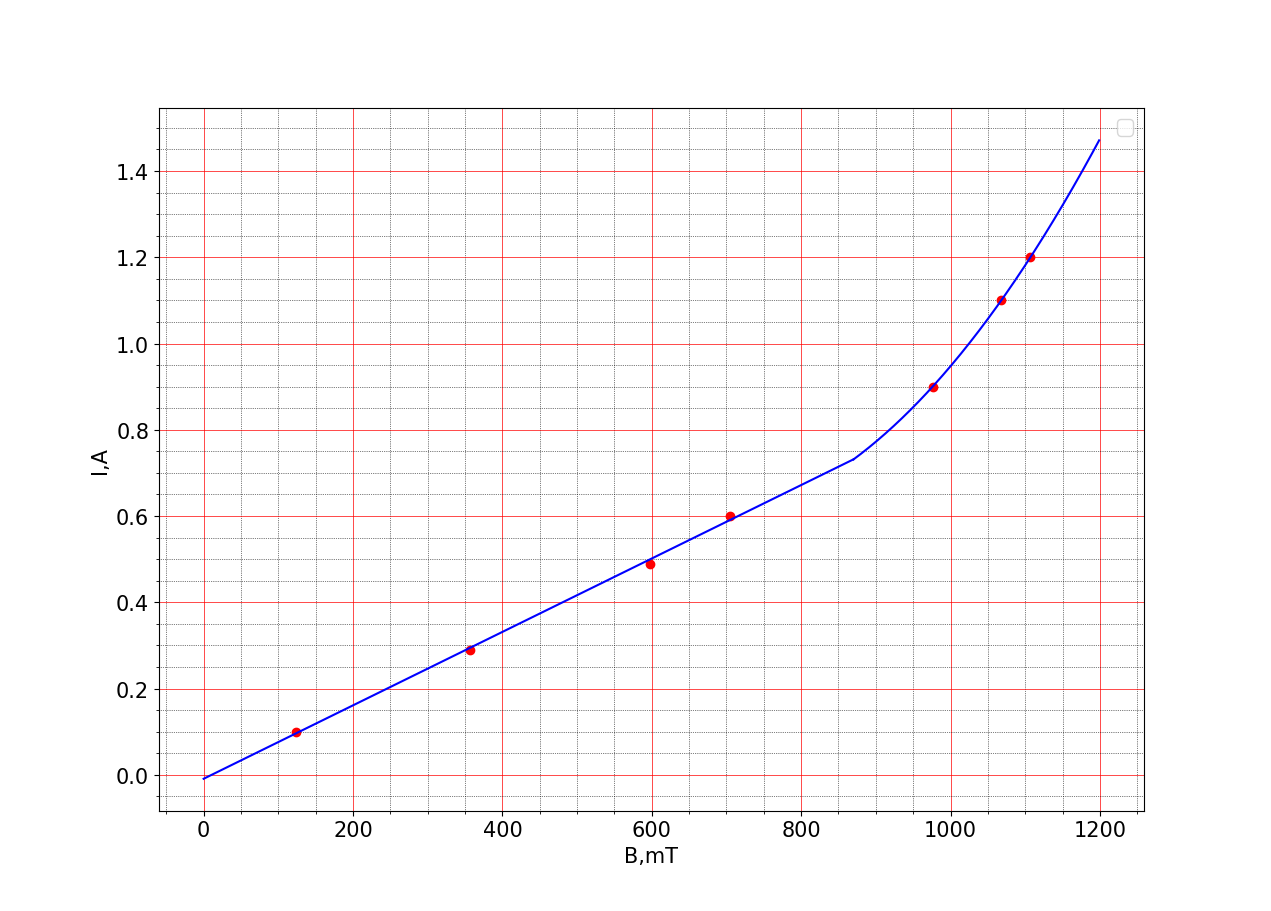
\includegraphics[width=0.9\linewidth]{Holl_1.png} 
    \caption{Калмбровочный график зависимости $B(I_m)$}
\end{figure}
Найдем ЭДС Холла и построим графики зависимостей U(B) для серебра и меди\\
\begin{tabular}{|l|l|l|l|l|l|l|l|l|l|l|l|l|l|l|}
\hline
\centering
Iобр,A    & 0.2  &       & 0.4       &      &      & 0.6       &      &      \\ \hline
U,0.04мкВ & Im,A & B,mT  & U,0.04мкВ & Im,A & BmT  & U,0.04мкВ & Im,A & BmT  \\ \hline
0         & 0    & 0     & -1.5      & 0    & 0    & -3        & 0    & 0    \\ \hline
1         & 0.1  & 123.3 & 1         & 0.2  & 245  & 1         & 0.2  & 240 \\ \hline
2         & 0.3  & 356   & 4         & 0.39 & 480  & 5         & 0.4  & 480 \\ \hline
3         & 0.6  & 705   & 6         & 0.6  & 705  & 8         & 0.6  & 705  \\ \hline
5         & 0.8  & 920   & 9         & 0.9  & 976  & 11        & 0.8  & 920 \\ \hline
6         & 1    & 1025  & 11        & 1.2  & 1107 & 13        & 1    & 1025 \\ \hline

\cline{1-9}
 0.8       &      &      & 1         &      &     \\ \hline
 U,0.04мкВ & Im,A & BmT  & U,0.04мкВ & Im,A & BmT  \\ \hline
 -5        & 0    & 0    & -7        & 0    & 0    \\ \hline
  0         & 0.2  & 240  & 0         & 0.2  & 240  \\ \hline
  5         & 0.4  & 480  & 6         & 0.4  & 480  \\ \hline
  10        & 0.6  & 705  & 12        & 0.6  & 705  \\ \hline
   15        & 0.8  & 920  & 18        & 0.8  & 920  \\ \hline
   17        & 1    & 1025 & 20        & 1    & 1025 \\ \hline
   
\end{tabular}
\begin{figure}
    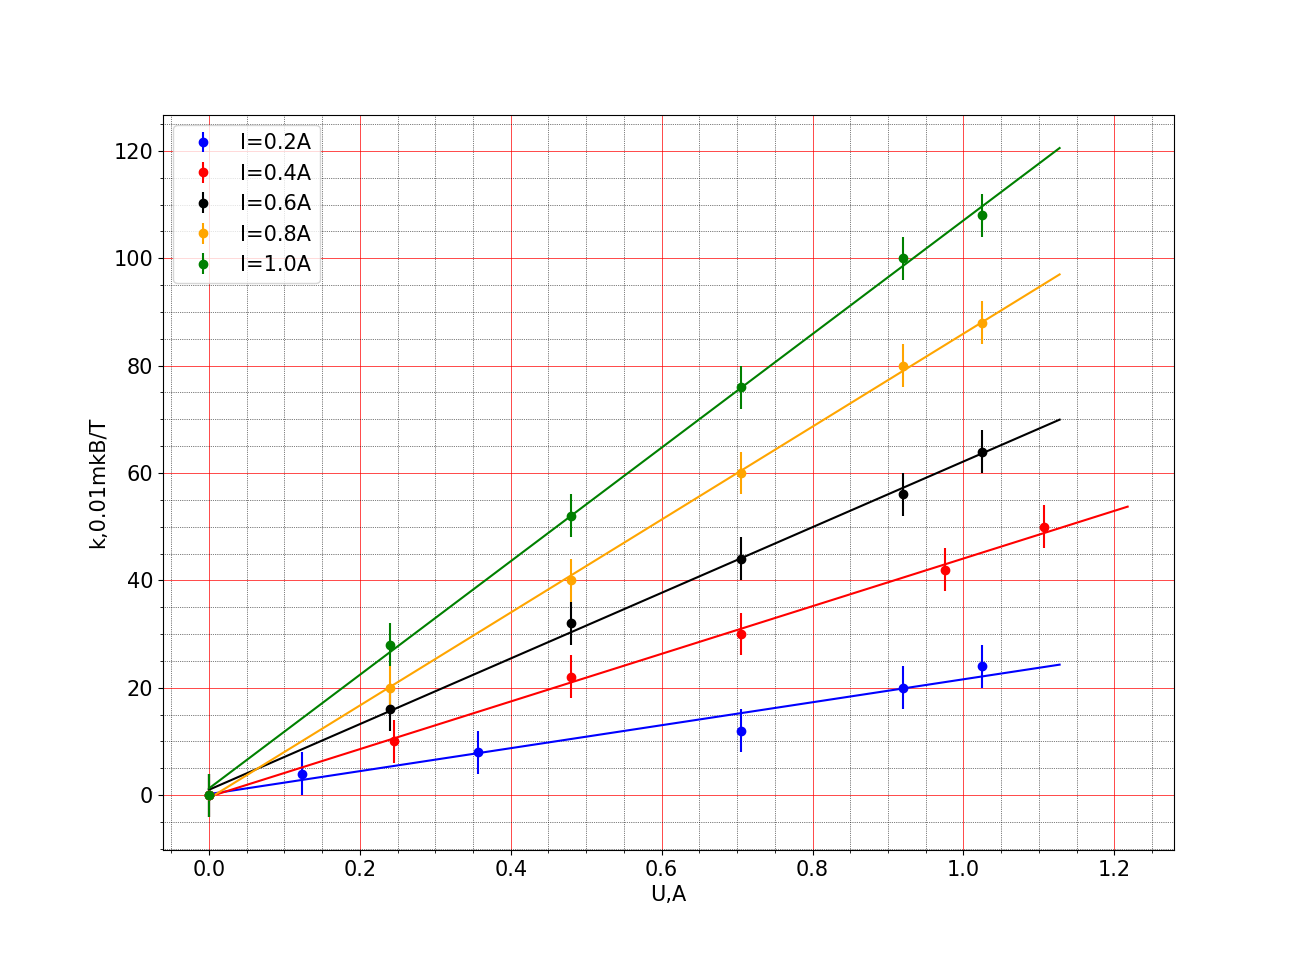
\includegraphics[width=1\linewidth]{Holl_2.png} 
    \caption{зависимость $U(B)$ для разных токов для серебра}
\end{figure}
\begin{table}
\begin{tabular}{|l|l|l|l|l|l|l|l|l|l|l|l|l|l|l|}
\hline
Iобр,A    & 0.2  &      & 0.4       &      &      & 0.6       &      &      \\ \hline
U,0.04mkB & Im,A & B,mT & U,0.04mkB & Im,A & B,mT & U,0.04mkB & Im,A & B,mT \\ \hline
7         & 0    & 0    & 6         & 0    & 0    & 6         & 0    & 0    \\ \hline
11        & 0.4  & 480  & 15        & 0.4  & 480  & 18        & 0.4  & 480  \\ \hline
13        & 0.6  & 705  & 17        & 0.6  & 705  & 25        & 0.6  & 705 \\ \hline
15        & 0.8  & 920  & 22        & 0.8  & 920  & 29        & 0.8  & 920 \\ \hline
16        & 1    & 1025 & 24        & 1    & 1025 & 32        & 1    & 1025 \\ \hline
17        & 1.2  & 1107 & 25        & 1.2  & 1107 & 35        & 1.2  & 1107 \\ \hline

\cline{1-9}

0.8       &      &      & 1         &      &      \\ \hline
 U,0.04mkB & Im,A & B,mT & U,0.04mkB & Im,A & B,mT \\ \hline
 6         & 0    & 0    & 7         & 0    & 0    \\ \hline
 22        & 0.4  & 480  & 26        & 0.4  & 480  \\ \hline
 30        & 0.6  & 705  & 37        & 0.6  & 705  \\ \hline
 38        & 0.8  & 920  & 46        & 0.8  & 920  \\ \hline
 41        & 1    & 1025 & 50        & 1    & 1025 \\ \hline
 44        & 1.2  & 1107 & 53        & 1.2  & 1107 \\ \hline
\end{tabular}
\end{table}
\begin{figure}
    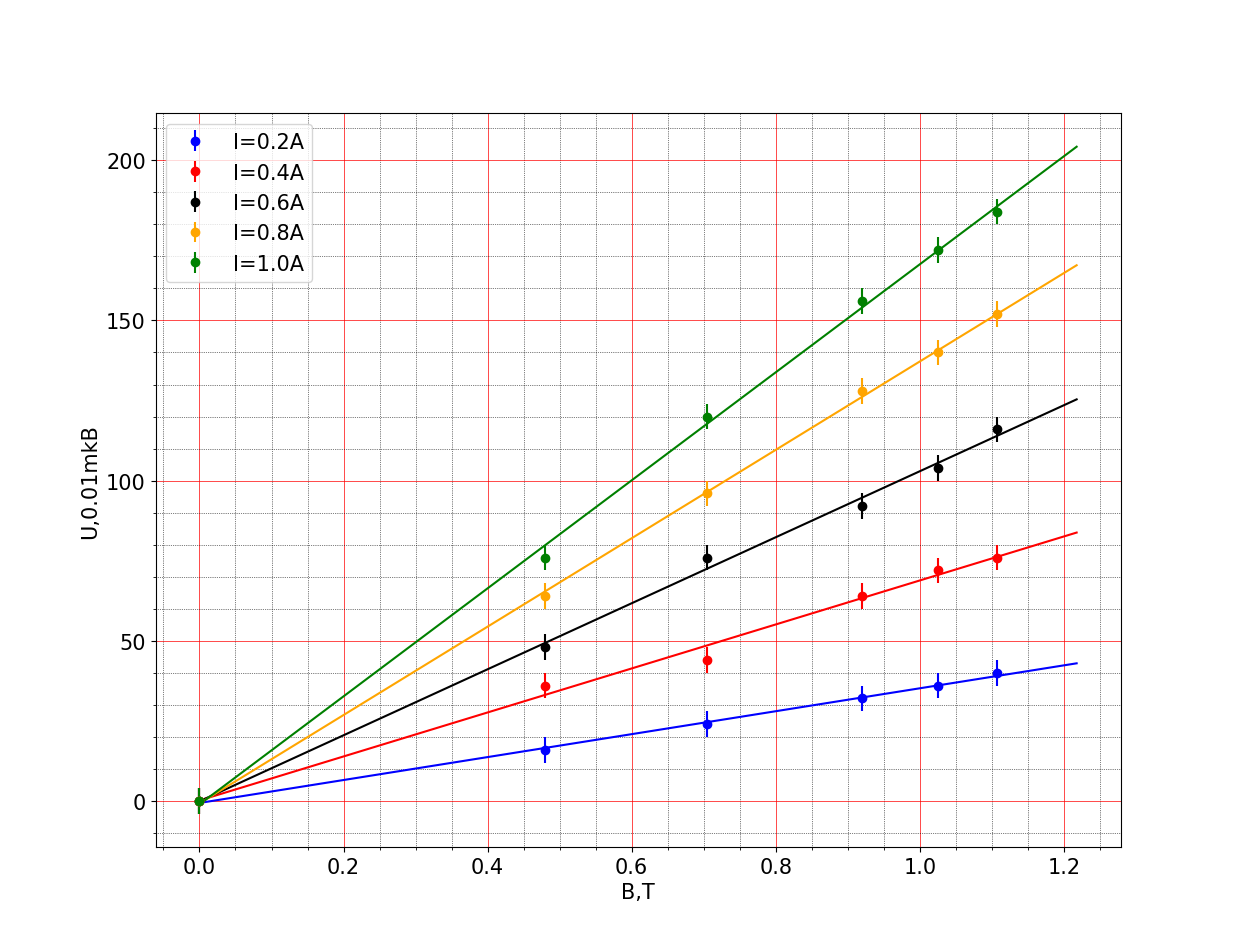
\includegraphics[width=1\linewidth]{Holl_3.png} 
    \caption{зависимость $U(B)$ для разных токов для меди}
\end{figure}
\begin{figure}
    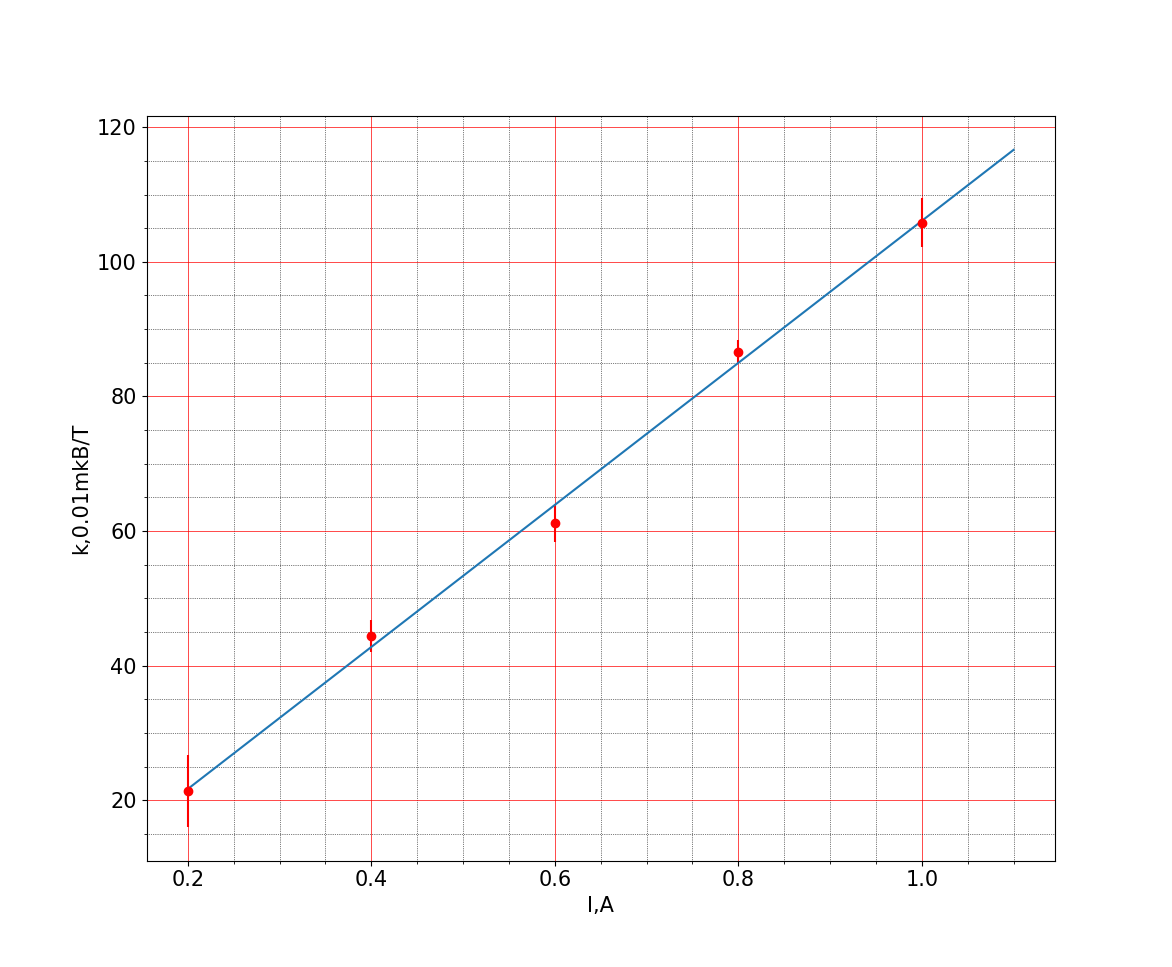
\includegraphics[width=0.8\linewidth]{Holl_4.png} 
    \caption{зависимость $k(I)$ для серебра}
\end{figure}
\begin{figure}
    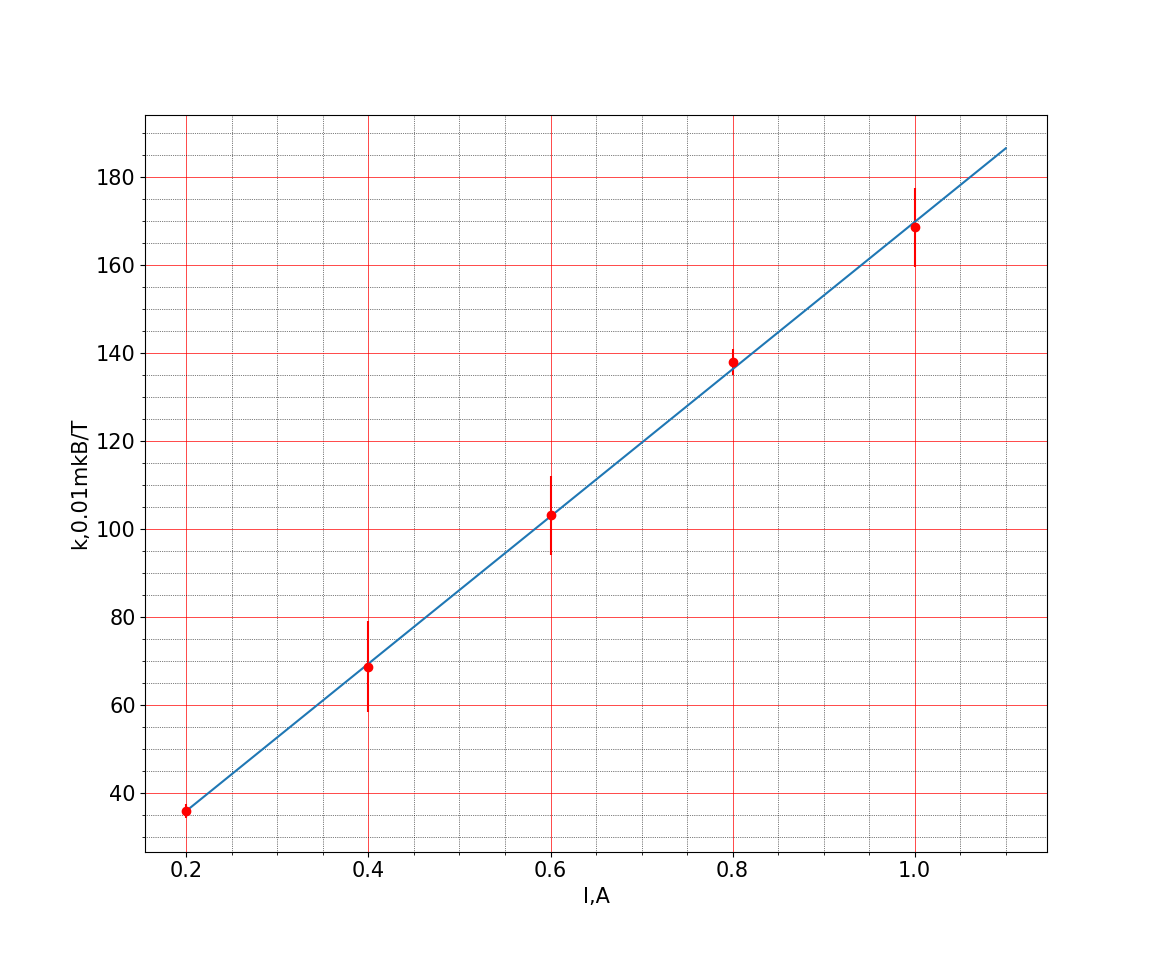
\includegraphics[width=0.8\linewidth]{Holl_5.png} 
    \caption{зависимость $k(I)$ для меди}
\end{figure}
\\
Найдя из графиков зависимости к(I) построим графики для серебра и меди
из них найдем $U\over{BI}$ и подставив в формулу 6 получим:
\[|R(Ar)| = (0.95 \pm  0.15)*10^{-10} {{m^3}\over{Kl}}\]
\[|R(Cu)| = (0.8 \pm  0.2)*10^{-10} {{m^3}\over{Kl}}\]
построим аналогичный график для цинка, правда только для I=1A\\
из графика для цинка найдем $R(Zn)$
\[|R(Zn)| = (1.3 \pm  0.3)*10^{-10} {{m^3}\over{Kl}}\]
\begin{figure}
    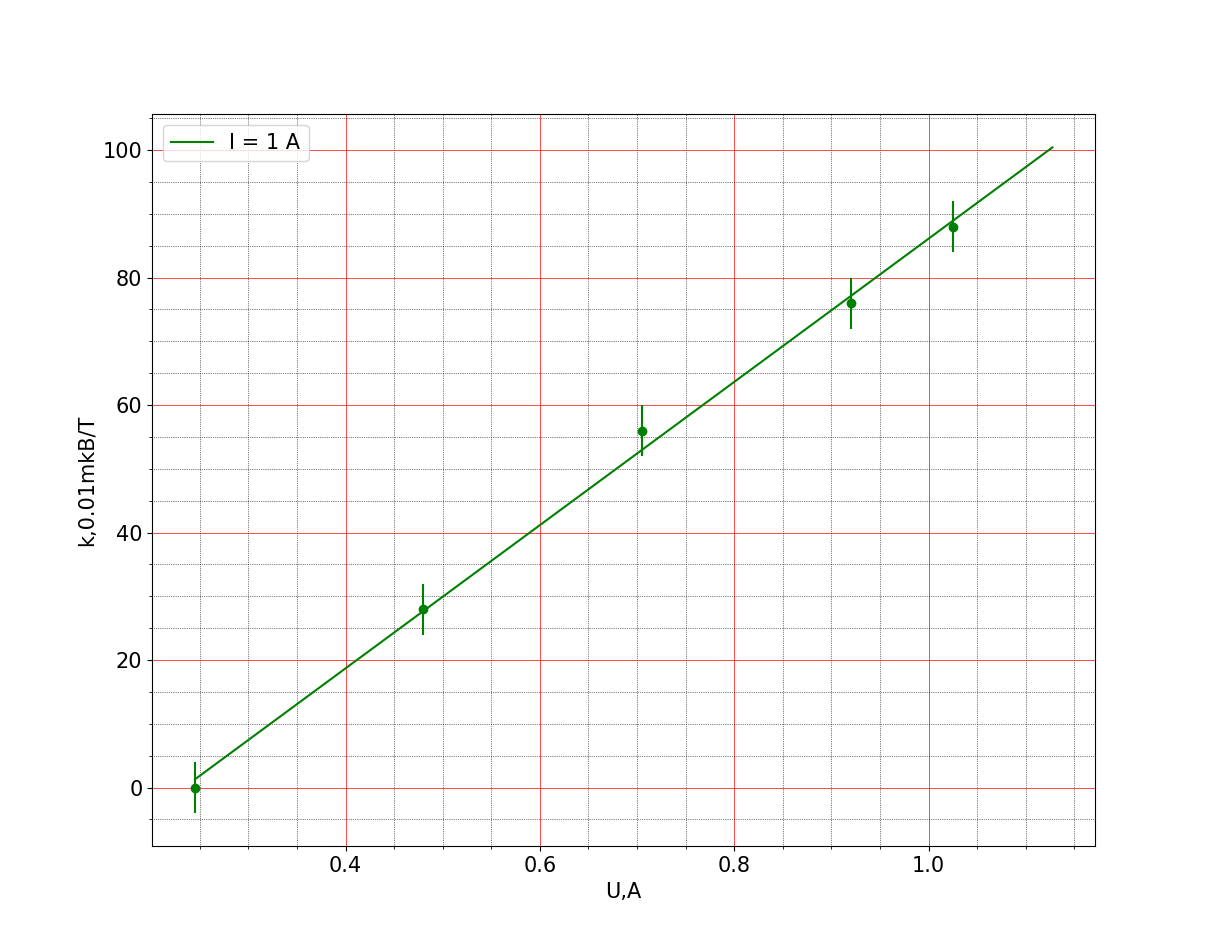
\includegraphics[width=0.8\linewidth]{Holl_6.png} 
    \caption{зависимость $U(B)$ для цинка}
\end{figure}
Для каждого из образцов рассчитаем концентрацию носителей тока $n$,удельную проводимость $\sigma_0$ и подвижность носителец тока $\mu $
\[n = {1\over{qR}}\]
\[\sigma_0 = {IL_{34}\over{U_{34}al}}\]
\[b = {\sigma_0\over{qn}}\]
\begin{table}
\begin{tabular}{|l|l|l|l|l|l|l|}
\hline
Металл & \begin{tabular}{l}$(R_h \pm \Delta R_h),$ \\ $10^{-10} {m^3\over{Kl}}$\end{tabular}& \begin{tabular}{l}табл $R_h,$ \\$ 10^{-10} {m^3\over{Kl}}$\end{tabular}&знак& \begin{tabular}{l}$(n \pm \Delta n),$\\$10^{28}m^{-3}$ \end{tabular}& \begin{tabular}{l}$(\sigma \pm \Delta \sigma),$\\$ 10^7(Om*m)^{-1}$ \end{tabular}&$ b {cm^2\over{B*c}}$\\ \hline
Ar     & $-(0.95 \pm  0.15) $&    -0.9   & -              & $-(6.5 \pm  1.0)$ & $(4.1 \pm  0.2) $     & $(40 \pm  8) $  \\ \hline
Cu     & $-(0.8 \pm  0.2) $& -0.55      & -             & $-(7.8 \pm  2.0)$ & $(3.9 \pm  0.2)$  & $(31 \pm  6)$ \\ \hline
Zn     & $(1.3 \pm  0.3) $& 1.04      & +            & $(4.8 \pm  1.1)$ & $(1.12 \pm  0.08)$     & $(15 \pm  3)$\\ \hline
\end{tabular}
\end{table}
\subsection*{Вывод}
Мы измерили некоторые постоянные металлов с точностью порядка $30\% $, значения напряжения оказались завышены, на это могло повлиять несколько факторов:
из-за некомпетентности лаборанта, магнитное поле менялось слишком быстро создавая дополнительное напряжение на образце,кроме того неизвестно с какой точностью были измерены 
параметры проводника, они могли внести дополнительную погрешность. Табличные данные брались из лабника, кроме цинка, для него данные из лабник отличались от данных из 
интернета в 2 раза.
\end{document}
